\documentclass{standalone}
\usepackage{tikz}
\usetikzlibrary{patterns, positioning}
\usepackage[sfdefault]{ClearSans} %% option 'sfdefault' activates Clear Sans as the default text font
\usepackage[T1]{fontenc}

\begin{document}
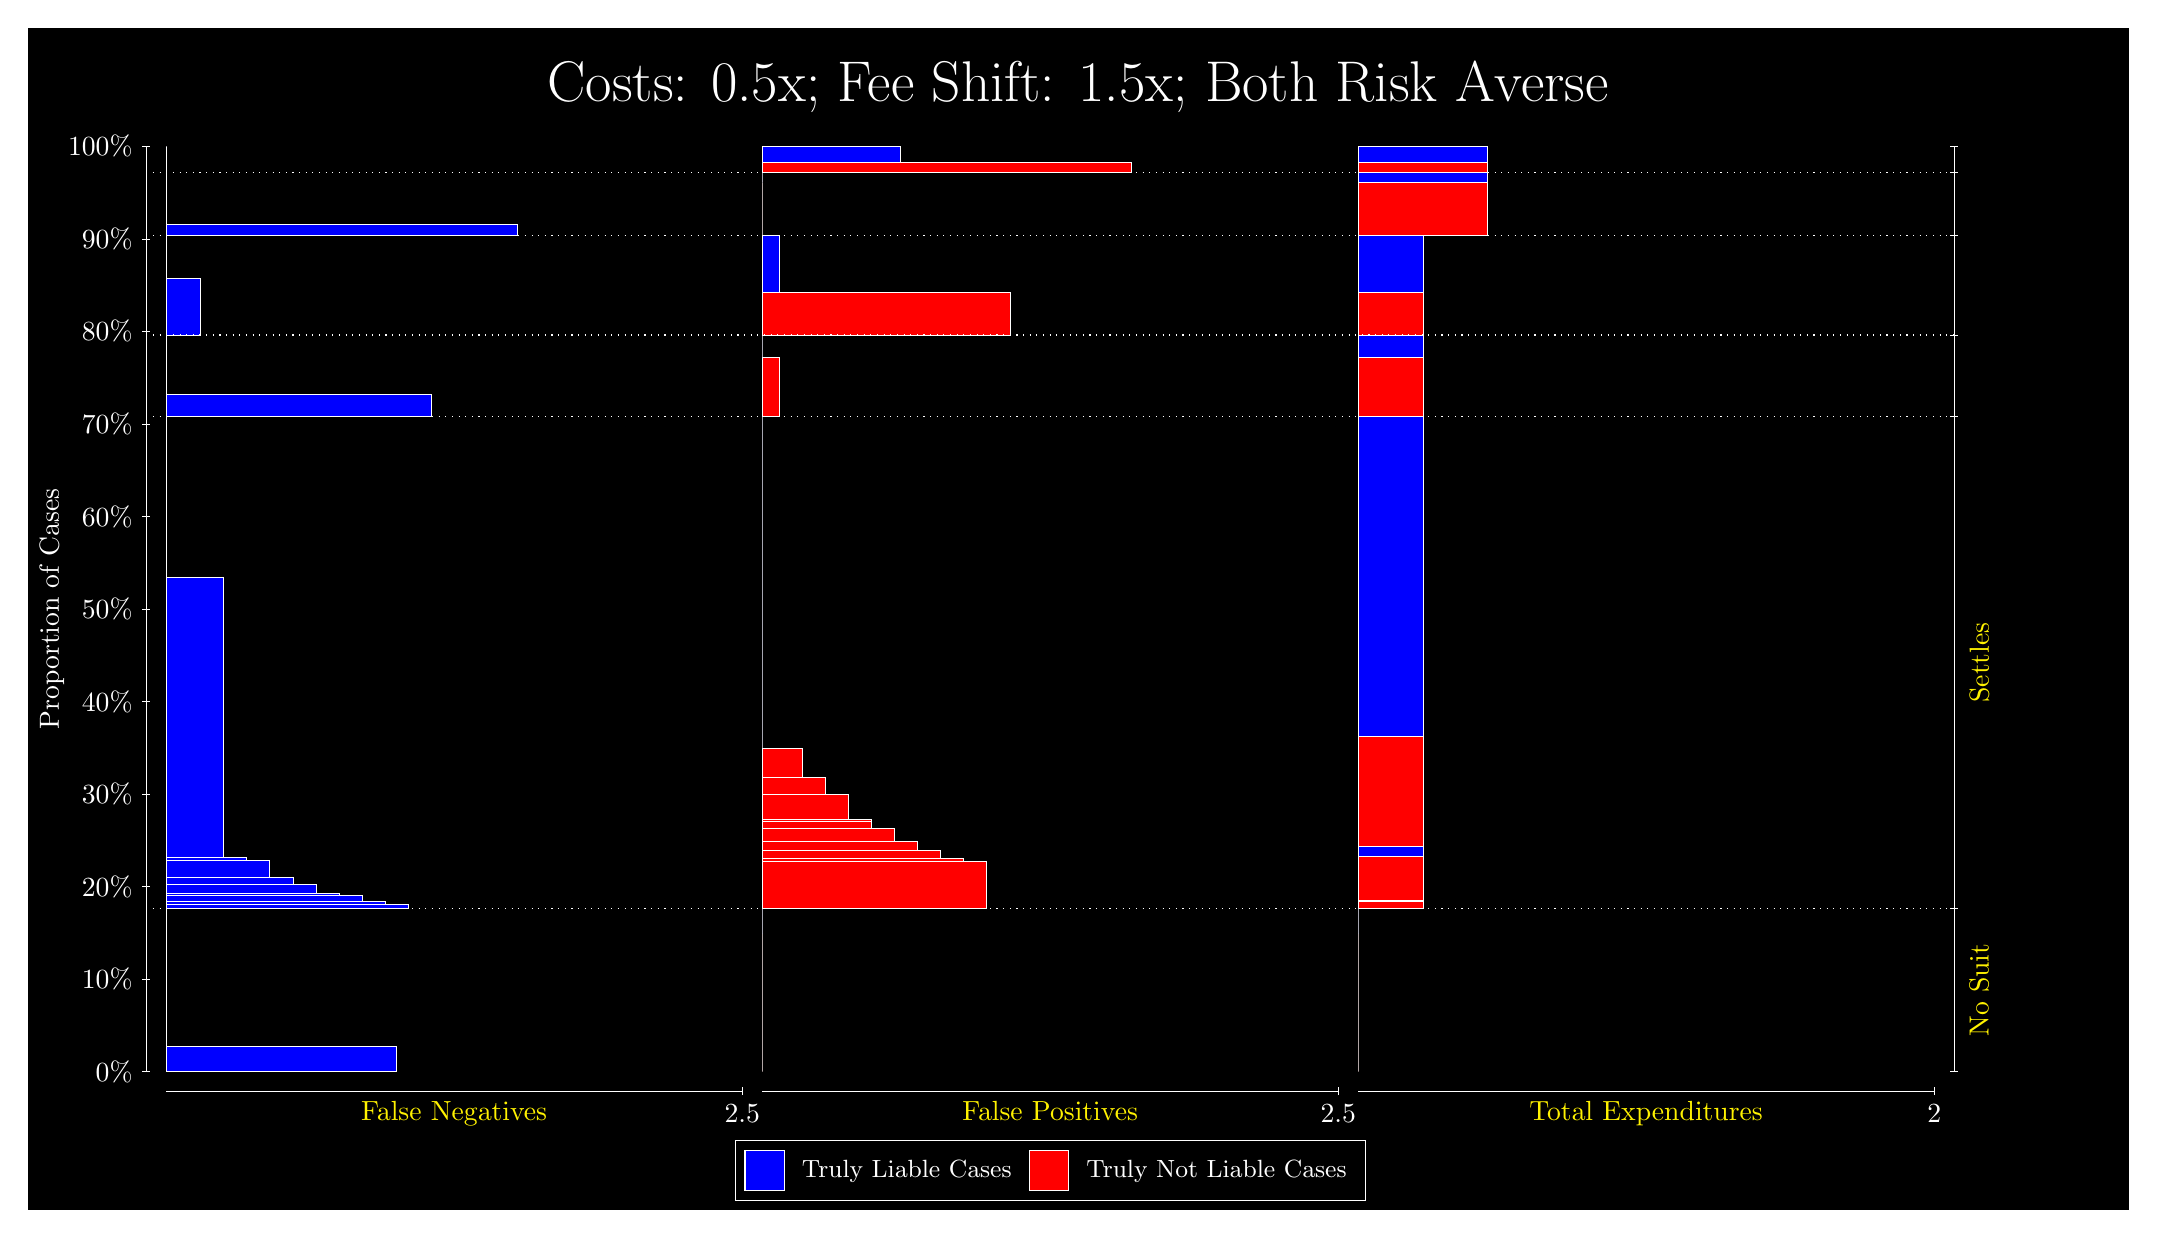
\begin{tikzpicture}
\draw[fill=black] (0,0) rectangle (26.667,15);
\draw[text=white] (0,13.5) rectangle (26.667,15) node[midway] {\huge Costs: 0.5x; Fee Shift: 1.5x; Both Risk Averse};
\draw[white, very thin] (1.5,1.75) -- (1.5,13.5);
\node[rotate=90, text=white, anchor=center] at (0.3, 7.625) {Proportion of Cases};
\draw[white, very thin] (1.45,1.75) -- (1.55,1.75);
\node[text=white, anchor=east] at (1.45, 1.75) {0\%};
\draw[white, very thin] (1.45,2.925) -- (1.55,2.925);
\node[text=white, anchor=east] at (1.45, 2.925) {10\%};
\draw[white, very thin] (1.45,4.1) -- (1.55,4.1);
\node[text=white, anchor=east] at (1.45, 4.1) {20\%};
\draw[white, very thin] (1.45,5.275) -- (1.55,5.275);
\node[text=white, anchor=east] at (1.45, 5.275) {30\%};
\draw[white, very thin] (1.45,6.45) -- (1.55,6.45);
\node[text=white, anchor=east] at (1.45, 6.45) {40\%};
\draw[white, very thin] (1.45,7.625) -- (1.55,7.625);
\node[text=white, anchor=east] at (1.45, 7.625) {50\%};
\draw[white, very thin] (1.45,8.8) -- (1.55,8.8);
\node[text=white, anchor=east] at (1.45, 8.8) {60\%};
\draw[white, very thin] (1.45,9.975) -- (1.55,9.975);
\node[text=white, anchor=east] at (1.45, 9.975) {70\%};
\draw[white, very thin] (1.45,11.15) -- (1.55,11.15);
\node[text=white, anchor=east] at (1.45, 11.15) {80\%};
\draw[white, very thin] (1.45,12.325) -- (1.55,12.325);
\node[text=white, anchor=east] at (1.45, 12.325) {90\%};
\draw[white, very thin] (1.45,13.5) -- (1.55,13.5);
\node[text=white, anchor=east] at (1.45, 13.5) {100\%};

\draw[white, very thin] (24.457,1.75) -- (24.457,13.5);
\draw[white, very thin] (24.407,1.75) -- (24.507,1.75);
\node[anchor=west] at (24.407, 1.75) {};
\draw[white, very thin] (24.407,3.819) -- (24.507,3.819);
\node[anchor=west] at (24.407, 3.819) {};
\draw[white, very thin] (24.407,10.071) -- (24.507,10.071);
\node[anchor=west] at (24.407, 10.071) {};
\draw[white, very thin] (24.407,11.104) -- (24.507,11.104);
\node[anchor=west] at (24.407, 11.104) {};
\draw[white, very thin] (24.407,12.372) -- (24.507,12.372);
\node[anchor=west] at (24.407, 12.372) {};
\draw[white, very thin] (24.407,13.172) -- (24.507,13.172);
\node[anchor=west] at (24.407, 13.172) {};
\draw[white, very thin] (24.407,13.5) -- (24.507,13.5);
\node[anchor=west] at (24.407, 13.5) {};

\draw[white, very thin, fill=blue] (1.75,1.75) rectangle (4.6775,2.0721);
\draw[white, very thin, fill=red] (1.75,2.0721) rectangle (1.75,3.819);
\draw[white, very thin, fill=blue] (1.75,3.819) rectangle (4.8239,3.8715);
\draw[white, very thin, fill=blue] (1.75,3.8715) rectangle (4.5312,3.9167);
\draw[white, very thin, fill=blue] (1.75,3.9167) rectangle (4.2384,3.987);
\draw[white, very thin, fill=blue] (1.75,3.987) rectangle (3.9457,4.0158);
\draw[white, very thin, fill=blue] (1.75,4.0158) rectangle (3.6529,4.1308);
\draw[white, very thin, fill=blue] (1.75,4.1308) rectangle (3.3602,4.2206);
\draw[white, very thin, fill=blue] (1.75,4.2206) rectangle (3.0674,4.432);
\draw[white, very thin, fill=blue] (1.75,4.432) rectangle (2.7746,4.4674);
\draw[white, very thin, fill=blue] (1.75,4.4674) rectangle (2.4819,8.0304);
\draw[white, very thin, fill=red] (1.75,8.0304) rectangle (1.75,10.071);
\draw[white, very thin, fill=blue] (1.75,10.071) rectangle (5.1167,10.357);
\draw[white, very thin, fill=red] (1.75,10.357) rectangle (1.75,11.104);
\draw[white, very thin, fill=blue] (1.75,11.104) rectangle (2.1891,11.829);
\draw[white, very thin, fill=red] (1.75,11.829) rectangle (1.75,12.372);
\draw[white, very thin, fill=blue] (1.75,12.372) rectangle (6.2145,12.505);
\draw[white, very thin, fill=red] (1.75,12.505) rectangle (1.75,13.172);
\draw[white, very thin, fill=red] (1.75,13.172) rectangle (1.75,13.303);
\draw[white, very thin, fill=blue] (1.75,13.303) rectangle (1.75,13.5);
\draw[white, very thin, fill=red] (9.3189,1.75) rectangle (9.3189,3.4969);
\draw[white, very thin, fill=blue] (9.3189,3.4969) rectangle (9.3189,3.819);
\draw[white, very thin, fill=red] (9.3189,3.819) rectangle (12.173,4.4234);
\draw[white, very thin, fill=red] (9.3189,4.4234) rectangle (11.88,4.4525);
\draw[white, very thin, fill=red] (9.3189,4.4525) rectangle (11.588,4.5614);
\draw[white, very thin, fill=red] (9.3189,4.5614) rectangle (11.295,4.6731);
\draw[white, very thin, fill=red] (9.3189,4.6731) rectangle (11.002,4.8453);
\draw[white, very thin, fill=red] (9.3189,4.8453) rectangle (10.709,4.9325);
\draw[white, very thin, fill=red] (9.3189,4.9325) rectangle (10.709,4.9567);
\draw[white, very thin, fill=red] (9.3189,4.9567) rectangle (10.417,5.2729);
\draw[white, very thin, fill=red] (9.3189,5.2729) rectangle (10.124,5.4908);
\draw[white, very thin, fill=red] (9.3189,5.4908) rectangle (9.8312,5.8593);
\draw[white, very thin, fill=blue] (9.3189,5.8593) rectangle (9.3189,10.071);
\draw[white, very thin, fill=red] (9.3189,10.071) rectangle (9.5384,10.818);
\draw[white, very thin, fill=blue] (9.3189,10.818) rectangle (9.3189,11.104);
\draw[white, very thin, fill=red] (9.3189,11.104) rectangle (12.466,11.647);
\draw[white, very thin, fill=blue] (9.3189,11.647) rectangle (9.5384,12.372);
\draw[white, very thin, fill=red] (9.3189,12.372) rectangle (9.3189,13.038);
\draw[white, very thin, fill=blue] (9.3189,13.038) rectangle (9.3189,13.172);
\draw[white, very thin, fill=red] (9.3189,13.172) rectangle (14.003,13.303);
\draw[white, very thin, fill=blue] (9.3189,13.303) rectangle (11.075,13.5);
\draw[white, very thin, fill=red] (16.888,1.75) rectangle (16.888,3.4969);
\draw[white, very thin, fill=blue] (16.888,3.4969) rectangle (16.888,3.819);
\draw[white, very thin, fill=red] (16.888,3.819) rectangle (17.711,3.9061);
\draw[white, very thin, fill=blue] (16.888,3.9061) rectangle (17.711,3.9293);
\draw[white, very thin, fill=red] (16.888,3.9293) rectangle (17.711,4.4875);
\draw[white, very thin, fill=blue] (16.888,4.4875) rectangle (17.711,4.6087);
\draw[white, very thin, fill=red] (16.888,4.6087) rectangle (17.711,6.0037);
\draw[white, very thin, fill=blue] (16.888,6.0037) rectangle (17.711,10.071);
\draw[white, very thin, fill=red] (16.888,10.071) rectangle (17.711,10.818);
\draw[white, very thin, fill=blue] (16.888,10.818) rectangle (17.711,11.104);
\draw[white, very thin, fill=red] (16.888,11.104) rectangle (17.711,11.647);
\draw[white, very thin, fill=blue] (16.888,11.647) rectangle (17.711,12.372);
\draw[white, very thin, fill=red] (16.888,12.372) rectangle (18.534,13.038);
\draw[white, very thin, fill=blue] (16.888,13.038) rectangle (18.534,13.172);
\draw[white, very thin, fill=red] (16.888,13.172) rectangle (18.534,13.303);
\draw[white, very thin, fill=blue] (16.888,13.303) rectangle (18.534,13.5);
\draw[white, dotted] (1.5,3.819) -- (24.457,3.819);
\draw[white, dotted] (1.5,10.071) -- (24.457,10.071);
\draw[white, dotted] (1.5,11.104) -- (24.457,11.104);
\draw[white, dotted] (1.5,12.372) -- (24.457,12.372);
\draw[white, dotted] (1.5,13.172) -- (24.457,13.172);
\draw[white, very thin] (1.75,1.5) -- (9.0689,1.5);
\node[text=yellow, anchor=north] at (5.4094, 1.5) {False Negatives};
\draw[white, very thin] (9.0689,1.45) -- (9.0689,1.55);
\node[text=white, anchor=north] at (9.0689, 1.45) {2.5};

\draw[white, very thin] (9.3189,1.5) -- (16.638,1.5);
\node[text=yellow, anchor=north] at (12.978, 1.5) {False Positives};
\draw[white, very thin] (16.638,1.45) -- (16.638,1.55);
\node[text=white, anchor=north] at (16.638, 1.45) {2.5};

\draw[white, very thin] (16.888,1.5) -- (24.207,1.5);
\node[text=yellow, anchor=north] at (20.547, 1.5) {Total Expenditures};
\draw[white, very thin] (24.207,1.45) -- (24.207,1.55);
\node[text=white, anchor=north] at (24.207, 1.45) {2};

\node[text=yellow, centered, rotate=90] at (24.777, 2.7845) {No Suit};
\node[text=yellow, centered, rotate=90] at (24.777, 6.9448) {Settles};





\draw (12.978300999999998,1.5) node[draw=none] (baseCoordinate) {};
\begin{scope}[align=center]
        \matrix[scale=0.5, draw=white, below=0.5cm of baseCoordinate, nodes={draw}, column sep=0.1cm]{
            \node[rectangle, draw, minimum width=0.5cm, minimum height=0.5cm, fill=blue] {}; &
            \node[draw=none, font=\small, text=white] (B) {Truly Liable Cases}; &
            \node[rectangle, draw, minimum width=0.5cm, minimum height=0.5cm, fill=red] {}; &
            \node[draw=none, font=\small, text=white] (B) {Truly Not Liable Cases}; \\
            };
\end{scope}

\end{tikzpicture}
\end{document}